\subsubsection{Self-supervised learning: training with simulated resections only}
\label{sec:self}

In our first experiment, we assess the relation between the resection simulation complexity and the segmentation performance of the model.
We train our model with simulated resections on the publicly available dataset $D\pre = \{ \X_{{\pre}_i} \}_{i = 1}^{n\pre}$, where $n\pre = 1813$ (\cref{sec:data}).
We use 90\% of the images in $D\pre$ for the training set $D\st{pre,train}$ and 10\% for the validation set.
At each training iteration, $b$ images from $D\st{pre,train}$ are loaded, resected, preprocessed and augmented to obtain a mini-batch of $b$ training instances
$\{ ( \X_{\text{sim}_i}, \Y_{\text{sim}_i}) \}_{i = 1}^{b}$.
Note that the resection simulation is performed on the fly, which ensures that the network never sees the same resection during training.
Models were trained for 60 epochs, using an initial learning rate of $10^{-3}$.
We use the model weights from the epoch with the lowest mean validation loss obtained during training for evaluation.
Models were tested on the 133 annotated images in EPISURG.

To investigate the effect of the simulated cavity shape on model performance, we modify $\phi\simul$ to generate cuboid- (\cref{fig:exp_shape_cuboid}) or ellipsoid-shaped (\cref{fig:exp_shape_ellipsoid}) resections, and compare with the baseline ``noisy'' ellipsoid (\cref{fig:exp_shape_noisy}).
The cuboids and ellipsoid meshes are not perturbed using simplex noise, and cuboids are not rotated.

Best results were obtained by the baseline model (80.5 (18.7)), trained using ellipsoids perturbed with procedural noise.
Models trained with cuboids and rotated ellipsoids performed significantly (57.9 (73.1), $p < 10^{-8}$) and marginally (79.0 (20.0), $p = 0.123$) worse.

\begin{figure}
  \centering
  \captionsetup[subfigure]{aboveskip=3pt, belowskip=5pt}

  \begin{subfigure}{0.32\textwidth}
    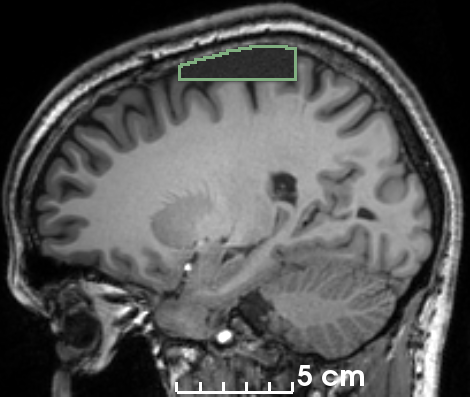
\includegraphics[width=\linewidth]{exp_shape_cuboid}
    \caption{\label{fig:exp_shape_cuboid}}
  \end{subfigure}
  \hfill
  \begin{subfigure}{0.32\textwidth}
    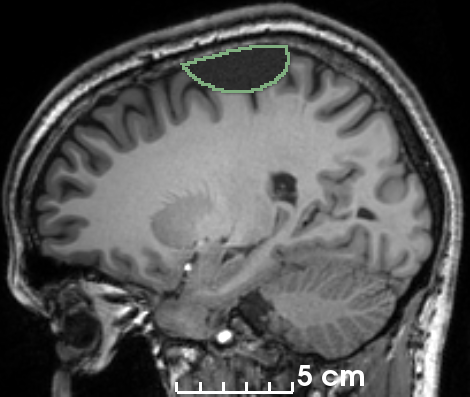
\includegraphics[width=\linewidth]{exp_shape_ellipsoid}
    \caption{\label{fig:exp_shape_ellipsoid}}
  \end{subfigure}
  \hfill
  \begin{subfigure}{0.32\textwidth}
    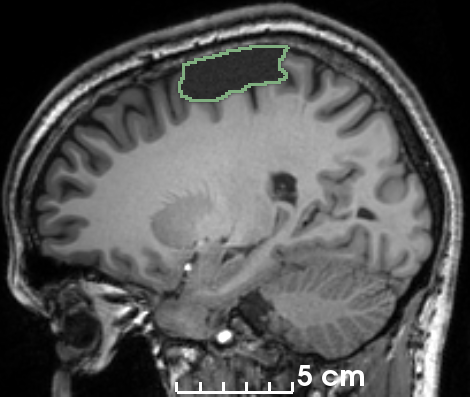
\includegraphics[width=\linewidth]{exp_shape_noisy}
    \caption{\label{fig:exp_shape_noisy}}
  \end{subfigure}

  \caption[Simulation of resection cavities with increasing complexity]{
    Simulation of resection cavities with increasing shape complexity (\cref{sec:simulation}):
    cuboid (\subref{fig:exp_shape_cuboid}),
    ellipsoid (\subref{fig:exp_shape_ellipsoid})
    and ellipsoid perturbed with simplex noise (\subref{fig:exp_shape_noisy}).
  }
  \label{fig:exp_shape}
\end{figure}
